\documentclass{article}
\usepackage{amsmath}
%%
%% Default settings for artisynth
%%
\NeedsTeXFormat{LaTeX2e}
%%\ProvidesPackage{artisynthDoc}[2012/04/05]

\usepackage[T1]{fontenc}
\usepackage[latin1]{inputenc}
\usepackage{listings}
\usepackage{makeidx}
\usepackage{latexml}
\usepackage{graphicx}
\usepackage{framed}
\usepackage{color}

\newcommand{\pubdate}{\today}
\newcommand{\setpubdate}[1]{\renewcommand{\pubdate}{#1}}

\iflatexml
\usepackage{hyperref}
\else
%% then we are making a PDF, so include things that LaTeXML can't handle: 
%% docbook style, \RaggedRight
\usepackage{ifxetex}
\usepackage{pslatex} % fixes fonts; in particular sets a better-fitting \tt font
\usepackage[hyperlink]{asciidoc-dblatex} 
%\usepackage{verbatim}
\usepackage{ragged2e}
\setlength{\RaggedRightRightskip}{0pt plus 4em}
\RaggedRight
\renewcommand{\DBKpubdate}{\pubdate}
\renewcommand{\DBKreleaseinfo}{}
\fi

% set hypertext links to be dark blue:
\definecolor{darkblue}{rgb}{0,0,0.8}
\definecolor{sidebar}{rgb}{0.5,0.5,0.7}
\hypersetup{colorlinks=true,urlcolor=darkblue,linkcolor=darkblue}

%%%%%%%%%%%%%%%%%%%%%%%%%%%%%%%%%%%%%%%%%%%%%%%%%%%%%%%%%%%%%%%%%%%%%%%%%%%%%
%
% Define macros for handling javadoc class and method references
%
%%%%%%%%%%%%%%%%%%%%%%%%%%%%%%%%%%%%%%%%%%%%%%%%%%%%%%%%%%%%%%%%%%%%%%%%%%%%%
\makeatletter

% code inspired by http://stackoverflow.com/questions/2457780/latex-apply-an-operation-to-every-character-in-a-string
\def\removeargs #1{\doremoveargs#1$\wholeString\unskip}
\def\doremoveargs#1#2\wholeString{\if#1$%
\else\if#1({()}\else{#1}\taketherest#2\fi\fi}
\def\taketherest#1\fi
{\fi \doremoveargs#1\wholeString}

% Note: still doesn't work properly when called on macro output ...
% i.e., \dottoslash{\concatnames{model}{base}{foo}} fails 
\def\dottoslash #1{\dodottoslash#1$\wholeString\unskip}
\def\dodottoslash#1#2\wholeString{\if#1$%
\else\if#1.{/}\else{#1}\fi\dottaketherest#2\fi}
\def\dottaketherest#1\fi{\fi \dodottoslash#1\wholeString}

% concatenates up to three class/method names together, adding '.' characters
% between them. The first and/or second argument may be empty, in which case
% the '.' is omitted. To check to see if these arguments are empty, we
% use a contruction '\if#1@@', which will return true iff #1 is empty
% (on the assumption that #1 will not contain a '@' character).
\def\concatnames
#1#2#3{\if#1@@\if#2@@#3\else #2.#3\fi\else\if#2@@#1.#3\else#1.#2.#3\fi\fi}

\newcommand{\javabase}{}
\newcommand{\setjavabase}[1]{\renewcommand{\javabase}{#1}}
\iflatexml
\newcommand{\javaclassx}[2][]{%
% Includes code to prevent an extra '.' at the front if #1 is empty. It
% works like this: if '#1' is empty, then '#1.' expands to '.', and so 
% '\if#1..' will return true, in which case we just output '#2'.
\href{@JDOCBEGIN/\concatnames{\javabase}{#1}{#2}@JDOCEND}{#2}}
\newcommand{\javaclass}[2][]{%
\href{@JDOCBEGIN/\concatnames{}{#1}{#2}@JDOCEND}{#2}}

\newcommand{\javamethodArgsx}[2][]{%
\href{@JDOCBEGIN/\concatnames{\javabase}{#1}{#2}@JDOCEND}{#2}}
\newcommand{\javamethodArgs}[2][]{%
\href{@JDOCBEGIN/\concatnames{}{#1}{#2}@JDOCEND}{#2}}

\newcommand{\javamethodNoArgsx}[2][]{%
\href{@JDOCBEGIN/\concatnames{\javabase}{#1}{#2}@JDOCEND}{\removeargs{#2}}}
\newcommand{\javamethodNoArgs}[2][]{%
\href{@JDOCBEGIN/\concatnames{}{#1}{#2}@JDOCEND}{\removeargs{#2}}}
\else
\def\javaurl{http://www.artisynth.org/doc/javadocs/}
\newcommand{\javaclassx}[2][]{{\color{darkblue}#2}}
%\href{\javaurl\dottoslash{\concatnames{\javabase}{#1}{#2}}.html}{#2}}
\newcommand{\javamethodArgsx}[2][]{{\color{darkblue}#2}}
\newcommand{\javamethodNoArgsx}[2][]{{\color{darkblue}\removeargs{#2}}}
\newcommand{\javaclass}[2][]{{\color{darkblue}#2}}
%\href{\javaurl\dottoslash{\concatnames{\javabase}{#1}{#2}}.html}{#2}}
\newcommand{\javamethodArgs}[2][]{{\color{darkblue}#2}}
\newcommand{\javamethodNoArgs}[2][]{{\color{darkblue}\removeargs{#2}}}
\fi

\newcommand{\javamethod}{\@ifstar\javamethodNoArgs\javamethodArgs}
\newcommand{\javamethodx}{\@ifstar\javamethodNoArgsx\javamethodArgsx}

%%%%%%%%%%%%%%%%%%%%%%%%%%%%%%%%%%%%%%%%%%%%%%%%%%%%%%%%%%%%%%%%%%%%%%%%%%%%%
%
% Define macros for sidebars
%
%%%%%%%%%%%%%%%%%%%%%%%%%%%%%%%%%%%%%%%%%%%%%%%%%%%%%%%%%%%%%%%%%%%%%%%%%%%%%

\iflatexml
\newenvironment{sideblock}{\begin{quote}}{\end{quote}}
\else
\usepackage[strict]{changepage}
\definecolor{sidebarshade}{rgb}{1.0,0.97,0.8}
\newenvironment{sideblock}{%
    \def\FrameCommand{%
    \hspace{1pt}%
    {\color{sidebar}\vrule width 2pt}%
    %{\vrule width 2pt}%
    {\color{sidebarshade}\vrule width 4pt}%
    \colorbox{sidebarshade}%
  }%
  \MakeFramed{\advance\hsize-\width\FrameRestore}%
  \noindent\hspace{-4.55pt}% disable indenting first paragraph
  \begin{adjustwidth}{}{7pt}%
  %\vspace{2pt}\vspace{2pt}%
}
{%
  \vspace{2pt}\end{adjustwidth}\endMakeFramed%
}
\fi

\iflatexml
\newenvironment{shadedregion}{%
  \definecolor{shadecolor}{rgb}{0.96,0.96,0.98}%
  \begin{shaded*}%
% Put text inside a quote to create a surrounding blockquote that
% will properly accept the color and padding attributes
  \begin{quote}%
}
{%
  \end{quote}%
  \end{shaded*}%
}
\else
\newenvironment{shadedregion}{%
  \definecolor{shadecolor}{rgb}{0.96,0.96,0.98}%
  \begin{shaded*}%
}
{%
  \end{shaded*}%
}
\fi

% Wanted to create a 'listing' environment because lstlisting is
% tedious to type and because under latexml it may need
% some massaging to get it to work properly. But hard to do
% because of the verbatim nature of listing
%\iflatexml
%\newenvironment{listing}{\begin{lstlisting}}{\end{lstlisting}}%
%\else
%\newenvironment{listing}{\begin{lstlisting}}{\end{lstlisting}}%
%\fi

\iflatexml\else
% fancyhdr was complaining that it wanted a 36pt header height ...
\setlength{\headheight}{36pt}
\fi


% abbreviation for backslash character
\newcommand\BKS{\textbackslash}

\makeatother


\setcounter{tocdepth}{5}
\setcounter{secnumdepth}{3}

\title{Writing Documentation for ArtiSynth}
\author{John Lloyd}
\setpubdate{July 24, 2012}
\iflatexml
\date{}
\fi

\begin{document}

\maketitle

\iflatexml{\large\pubdate}\fi

\tableofcontents

\section{Introduction}

This document describes how to write and modify the main ArtiSynth
documentation set. It explains where the documentation sources are
kept, how they are converted into HTML or PDF files, what external
software is required, and what special conventions are used.

In addition to the main documentation described here, there may be
additional documentation available at
\href{http://www.artisynth.org}{www.artisynth.org}.

\section{How Documents Are Created}

ArtiSynth documentation is written using LaTeX, and converted into
either PDF output using {\tt pdflatex}, or HTML using LaTeXML
(\href{http://dlmf.nist.gov/LaTeXML/}{dlmf.nist.gov/LaTeXML}).  See
Section \ref{ExternalSoftwareSec} for instructions on installing LaTeXML.

{\tt Makefile}s are used to organize the commands and options needed
to create these different outputs.

The format for PDF output is based on that used by the
\href{http://www.docbook.org}{DocBook} project, while style for
HTML files is based on that used by
\href{http://www.methods.co.nz/asciidoc}{AsciiDoc}.

\subsection{Document Source Code Organization}

The sources for the various books and articles that make up the
documentation are located in subdirectories in {\tt
\$ARTISYNTH\_HOME/doc}.  For example, the sources for this document
are located in {\tt \$ARTISYNTH\_HOME/doc/documentation}, and the
source file itself is called {\tt documentation.tex}. 
By convention, if a
document contains images, then its image files are stored in a
sub-directory called {\tt images}.

Additional subdirectories of {\tt doc} include:

\begin{description}

\item[{\tt misc/} ] \mbox{}

Contains miscellaneous and older documentation in formats, including
text files.

\item[{\tt javadocs/} ] \mbox{}

Contains the Javadoc API documentation.

\item[{\tt html/} ] \mbox{}

Contains the HTML output produced by LaTeXML.

\item[{\tt texinputs/} ] \mbox{}

Contains input and style files used by LaTeX.

\item[{\tt style/} ] \mbox{}

Contains CSS style sheets.

\end{description}

\subsection{Document Creation Commands}

Each documentation source directory contains a {\tt Makefile}, which
implements a few basic commands to create PDF and/or HTML output files
from the LaTeX source files.  To use the {\tt Makefile} commands, you
need to be on a system that supports {\it GNU make}. This includes
Linux, MacOS, and Windows with Cygwin installed.

\subsection{HTML Output}

To create HTML output for a particular source document,
run the command
%
\begin{verbatim}
  > make html
\end{verbatim}
%
within that document's source directory. This will create the HTML
output and place it in a subdirectory under 
{\tt \$ARTISYNTH\_HOME/doc/html}. It will also
copy over any required image files.

\subsection{PDF Output}

To create PDF output for a document, you can use the command
%
\begin{verbatim}
  > make pdf
\end{verbatim}
%
The resulting PDF file is copied into the directory 
{\tt \$ARTISYNTH\_HOME/doc/pdf}.

%\subsection{Chunked HTML Output}
%
%Some documents can also be broken up into "chunked" HTML,
%with one chapter per HTML page. For those, the command
%
%\begin{verbatim}
%  > make chunked
%\end{verbatim}
%
%will create the chunked output and place it in
%a subdirectory under {\tt ../html}. As with {\tt make html}, image
%file sources are copied into a subdirectory under {\tt ../html}.
%
%\begin{sideblock}
%The usual workflow when editing or changing an ArtiSynth document is:
%
%- Edit the {\tt .txt} file in a regular text editor
%- Run {\tt make html} (or {\tt make pdf} or {\tt make chunked}) to create output
%- Examine the output using a browser or PDF reader
%\end{sideblock}

\subsection{Other Commands}

By way the {\tt make} operates, output will usually only be generated when
the output file does not exist or when it's older than the
corresponding {\tt .tex} source file. To ensure execution of a particular
{\tt make} command, you can precede it with
%
\begin{verbatim}
  > make clean
\end{verbatim}
%
which will remove all extraneous and output files.

There is also a {\tt Makefile} in {\tt \$ARTISYNTH\_HOME/doc} that
provides global {\tt make} commands for working on all the
documents. Within {\tt \$ARTISYNTH\_HOME/doc}, the command
%
\begin{verbatim}
  > make HTML
\end{verbatim}
%
(note the capitalization) will produce HTML output for
all the documents. Likewise, {\tt make PDF} 
will create all PDF output, and
%
\begin{verbatim}
  > make CLEAN
\end{verbatim}
%
will clean all the subdirectories. To copy the documentation
into a web-accessible directory, you can use
%
\begin{verbatim}
  > make webinstall
\end{verbatim}
%
which assumes that the variable {\tt WEBINSTALL\_DIR} is properly
set in the {\tt Makefile}.

To create the Javadocs, you can use
%
\begin{verbatim}
  > make javadocs
\end{verbatim}
%
which will use {\tt javadoc} to build the API documentation from
the system sources and place this in the {\tt javadoc} subdirectory.

\section{Installing Documents on the Webserver}
\label{InstallingSec}

Once you have created documentation, you may want to install it on the
ArtiSynth webserver. In order to do this, you need

\begin{enumerate}
\item an account on the ArtiSynth webserver (which is
currently {\tt www.magic.ubc.ca});
\item the environment variable {\tt ARTISYNTH\_WEB\_ACCOUNT} set to
the name of your account on that server;
\item {\tt ssh} and {\tt rsync} installed on your local machine.
\end{enumerate}

Then, from within a given documentation subdirectory, the {\tt make}
command
%
\begin {verbatim}
  > make install_html
\end{verbatim}
%
will create the HTML output associated with that directory and install
it on the ArtiSynth webserver. Likewise, the command
%
\begin {verbatim}
  > make install_pdf
\end{verbatim}
%
will create and install the PDF output.

You can also install {\it all} the HTML and PDF documentation 
by running 
%
\begin {verbatim}
  > make install_html
  > make install_pdf
\end{verbatim}
%
from the main documentation directory {\tt \$ARTSIYNTH\_HOME/doc}.

Also, from within {\tt \$ARTSIYNTH\_HOME/doc}, the command
%
\begin{verbatim}
  > make install_javadocs
\end{verbatim}
%
will install the Javadocs. Note that {\tt install\_javadocs} assumes you
have already built the Javadocs, which you can do using the command
%
\begin{verbatim}
  > make javadocs
\end{verbatim}
%
\begin{sideblock}
All of these installation commands work by using {\tt rsync}
to copy the files and
{\tt ssh} to then correctly set the permissions of the copied files.
Unfortunately, this means that you will probably have to enter your
webserver password twice.  
\end{sideblock}

\section{LaTeX usage and conventions}

\label{LatexUsage}

\subsection{LaTeXML restrictions}

All documentation is written in LaTeX, and conversion to HTML is done
via \href{http://dlmf.nist.gov/LaTeXML/}{LaTeXML}.  The latter is a
Perl-based application which translates a {\tt .tex} file into an XML
schema, which is then translated to HTML using XSLT. Currently,
version 0.8.0 or higher of LaTeXML is required; see 
Section \ref{ExternalSoftwareSec}.

LaTeXML is an ongoing project which was originally developed to
provide reliable conversion of LaTeX-based mathematical documents into
HTML and XHTML. It supports a large number of the more commonly used
LaTeX packages but does not support them all. Therefore, in some
circumstance, it may be useful to conditionalize the LaTeX source to
use different input depending on whether HTML or PDF output is being
produced. Producing HTML implies the use of LaTeXML, which can be
detected using the {\tt \BKS iflatexml} conditional, as in:

\begin{lstlisting}[]
\iflatexml
  do things in a conventional way that LaTeXML can deal with
\else
  \fancydancy{use some LaTeX package that LaTeXML can't handle}
\fi
\end{lstlisting}

Some specific problems with LaTeXML at the time of this writing
(May 2012) include:

\begin{itemize}

\item When specifying a font inside a list item, it is sometimes
necessary to include an extra space after the right closing brace,
as in
\begin{verbatim}
  \item[{\tt labelForItem} ]
\end{verbatim}
in order to prevent the font from spilling over into the body
of the item.

\item LaTeXML does not place the title page date (specified using {\tt
\BKS date\{\}}) on the titlepage. Instead, it is placed in the
footer at the page bottom. As a work-around, we use {\tt \BKS iflatex} to
leave {\tt \BKS date} empty and then place an explicit date at the top of
the page.

\item Blank lines are not properly handled in the {\tt lstlisting}
environment. This is fixed by post-processing the HTML output, as
described in Section \ref{LocalCustomizationSec}.

\item Some characters and character sequences (such as quotes, and the
sequence {\tt ...}) are converted into special unicode characters.
This actually reduces the readablity of code blocks, and so
post-processing is used to replace the unicode characters with the
orginals (Section \ref{LocalCustomizationSec}).

\end{itemize}

\subsection{Font conventions}

Programmatic literals, such as class and method names, file names, 
command sequences, and
environment variables are typeset in {\tt monospace}, using {\tt
\{\BKS tt monospace\}}. User interface literals, such as menu items, are
typeset in {\sf sans-serif}, using {\tt \{\BKS sf sans-serif\}}.

\subsection{Code blocks}

Small code blocks (typically one-line) are usually typeset using the
{\tt verbatim} environment, which produces output like this:

\begin{verbatim}
  > short one line code or command line example
\end{verbatim}

Longer code examples are typeset using the {\tt lstlisting}
environment (from the {\tt listings} package), which surrounds
the output in a colored box:

\begin{lstlisting}[]
// Here is a longer code example
interface Property
{
   Object get(); 
   void set (Object value); 
   Range getRange ();
   HasProperties getHost();
   PropertyInfo getInfo();
}
\end{lstlisting}

\subsection{Side blocks}
\label{SideBlocksSec}

A special environment called {\tt sideblock} is used to create
admonition sections that contain special notes, warnings, or side
information. The LaTeX source

\begin{lstlisting}[]
\begin{sideblock}
Note: when producing PDF, the {\tt sideblock} environment
is implemented using commands from the {\tt color} and
{\tt framed} packages. When producing HTML output, side blocks
are implemented internally using the
regular {\tt quote} environment, with the final appearance arranged
using the CSS stylesheet. 
\end{sideblock}
\end{lstlisting}

will produce output that looks like this:

\begin{sideblock}
Note: when producing PDF, the {\tt sideblock} environment
is implemented using commands from the {\tt color} and
{\tt framed} packages. When producing HTML output, side blocks
are implemented internally using the
regular {\tt quote} environment, with the final appearance arranged
using the CSS stylesheet. 
\end{sideblock}

\subsection{Inserting Images}

Image files are input using {\tt \BKS includegraphics} from the {\tt
graphics} package. 

Any type of image file can be used that is acceptable to {\tt
pdflatex} (e.g., {\tt .png}, {\tt .pdf}, and {\tt .jpg}). When creating
HTML output, LaTeXML automatically copies the image files into the
HTML target directory, converting them if necessary into a format
acceptable for web display (typically {\tt .png} or {\tt .jpg}). This
conversion is done using the
\href{http://www.imagemagick.org}{ImageMagic} application suite.

In some cases, good image appearance may require different image
scalings, depending on whether HTML or PDF output is being
produced. This is often true in particular for {\tt .png} files, where
for HTML one may not want any scaling at all (in order to get
pixel-for-pixel reproduction). This can be achieved using
{\tt \BKS iflatexml}:

\begin{lstlisting}[]
\begin{figure}
\begin{center}
\iflatexml
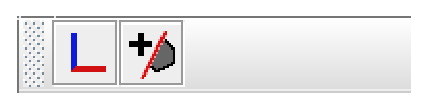
\includegraphics[]{images/viewerToolbar}
\else
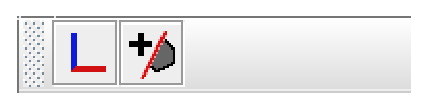
\includegraphics[width=2.5in]{images/viewerToolbar}
\fi
\end{center}
\caption{The viewer toolbar.}%
\end{lstlisting}

\subsection{Javadoc References}
\label{JavadocRefsSec}

ArtiSynth is implemented in Java, and so much of the documentation
refers to various Java classes and methods. It is therefore useful to
include hyperlinks from the documentation to the actual Javadoc pages.
Unfortunately, creating such a hyperlink can be rather tedious: If the
Javadocs are rooted at {\tt http://www.artisynth.org/doc/javadocs},
then a hyperlink to the class definition for {\tt
maspack.matrix.MatrixNd} must take the lengthy form
\begin{verbatim}
  \href{http://www.artisynth.org/doc/javadocs/maspack/matrix/MatrixNd.html}{MatrixNd}
\end{verbatim}
Method references are even worse, particularly if they contain arguments:
\begin{verbatim}
  \href{http:// ... MatrixNd.html#mul(maspack.matrix.MatrixNd)}{MatrixNd.mul()}
\end{verbatim}
To alieviate these problems, several LaTeX macros are provided that
build Javadoc references automatically from simple class and
method descriptions.

\subsubsection{Class references}
\label{ClassRefsSec}

The command {\tt \BKS javaclass} will create a Javadoc reference to 
a class from the class name itself. The LaTeX source

\begin{lstlisting}[]
\javaclass{maspack.matrix.MatrixNd}, and \javaclass[maspack]{matrix.MatrixNd}, and
\javaclass[maspack.matrix]{MatrixNd}.
\end{lstlisting}

will produce the output

\javaclass{maspack.matrix.MatrixNd}, and \javaclass[maspack]{matrix.MatrixNd}, and
\javaclass[maspack.matrix]{MatrixNd}.

The name in the optional argument (between square brackets {\tt []})
is prepended to the main argument to create a fully qualified class name,
with only the main argument being used as the anchor text. 

The names provided by the optional argument and the main argument are
concatenated (with an intervening '{\tt .}' character) to create a
fully qualified class name that is used to produce the appropriate
hyperlink to the Javadoc. For additional brevity in the LaTeX source
file, one can also use the command {\tt \BKS javaclassx}, which
internally prepends a package name provided by the expansion of {\tt
\BKS javabase} onto the class name. {\tt \BKS javabase} can be set
using the command {\tt \BKS setjavabase}, thus removing the need to
explicly specify the full class name in the arguments to {\tt \BKS
javaclassx}. For example,

\begin{lstlisting}[]
\setjavabase{maspack.matrix}
Two important classes are \javaclassx{MatrixNd} and \javaclassx{VectorNd}.
\end{lstlisting}

will produce the output

\setjavabase{maspack.matrix}
Two important classes are \javaclassx{MatrixNd} and \javaclassx{VectorNd}.

\subsubsection{Method references}

Methods can be referenced in a similar way using the command {\tt
\BKS javamethod}, which takes a class name plus the name of a method and
a (possibly abbreviated) argument signature.
LaTeX source of the form

\begin{lstlisting}[]
\javamethod{maspack.matrix.MatrixNd.mul()}, 
\javamethod[maspack.matrix]{MatrixNd.mul(MatrixNd)},
\javamethod[maspack.matrix.MatrixNd]{mul(MatrixNd,MatrixNd)}.
\end{lstlisting}

will produce output of the form

\setjavabase{}
\javamethod{maspack.matrix.MatrixNd.mul()}, 
\javamethod[maspack.matrix]{MatrixNd.mul(MatrixNd)},
\javamethod[maspack.matrix.MatrixNd]{mul(MatrixNd,MatrixNd)}.

As with {\tt \BKS javaclass}, an alternate method {\tt \BKS
javamethodx} is available which internally prepends the package name
provided by the expansion of {\tt \BKS javabase} onto the class name,
so that

\begin{lstlisting}[]
\setjavabase{maspack.matrix}
\javamethodx[MatrixNd]{mul(MatrixNd)} takes one argument,
while \javamethodx[MatrixNd]{mul(MatrixNd,MatrixNd)} takes two.
\end{lstlisting}

will produce output of the form

\setjavabase{maspack.matrix}
\javamethodx[MatrixNd]{mul(MatrixNd)} takes one argument,
while \javamethodx[MatrixNd]{mul(MatrixNd,MatrixNd)} takes two.

The argument signature does not need to contain the fully qualified
type names of the arguments. In fact, if the method name is unique to
the class, no argument list is needed at all; a simple {\tt ()} will
suffice.  Otherwise, if the method is overloaded, the argument
signature should be composed of comma-separated entries, each of which
partly matches the fully qualified type name of each argument.

For example,

\begin{lstlisting}[]
\javamethodx{MatrixNd.mul(maspack.matrix.MatrixNd,maspack.matrix.MatrixNd)}, 
\javamethodx{MatrixNd.mul(matrix.MatrixNd,matrix.MatrixNd)},
\javamethodx{MatrixNd.mul(MatrixNd,MatrixNd)}.
\end{lstlisting}

will all produce references to the same method. In fact, if the method
name and argument count is unique, then a set of commas indicating the
number of arguments will be sufficient, as in {\tt
\BKS javamethodx{MatrixNd.mul(,)}}.

Finally, to omit the argument signature from
the anchor text, one can use the commands {\tt \BKS javamethod*}
or {\tt \BKS javamethodx*} instead, so that

\begin{lstlisting}[]
Method reference with argument signature:
\javamethodx{MatrixNd.mul(MatrixNd,MatrixNd)}, and without:
\javamethodx*{MatrixNd.mul(MatrixNd,MatrixNd)}.
\end{lstlisting}

will produce the output

Method reference with argument signature:
\javamethodx{MatrixNd.mul(MatrixNd,MatrixNd)}, and without:
\javamethodx*{MatrixNd.mul(MatrixNd,MatrixNd)}.

\subsubsection{How it works}

{\tt \BKS javaclass} and {\tt \BKS javamethod} both work by creating a call
to {\tt \BKS href} with a place-holder link of the form

 {\tt \{@JDOCBEGIN /}{\it classOrMethodName} {\tt @JDOCEND\}}

This propagates to the output HTML file, which is then processed by
the Perl script {\tt setJavadocLinks} (located in {\tt
\$ARTISYNTH\_HOME/bin}) to convert '{\tt .}' characters to '{\tt /}'
characters, prepend the appropriate root link for the Javadocs (such
as {\tt http://www.\-artisynth.org/doc/javadocs}), and, for methods,
find and append the appropriate suffix to locate the method within the
class's Javadoc file.

\begin{sideblock}
{\bf Note:}\\
At present, working hyperlinks are only produced for HTML output.
Links are not produced for PDF output because of the difficulty
in performing these postprocessing functions in LaTeX itself.
\end{sideblock}

\section{Adding a New Document}

If you're adding a completely new document (as opposed
to modifying an existing one), then you should create a
new source directory for that document under {\tt \$ARTISYNTH\_HOME/doc},
and place the relevant {\tt .tex} files there.

\subsection{Creating and Updating the Makefiles}

You should also create a {\tt Makefile} in the new directory. This is most
easily done by copying an existing {\tt Makefile} from a similar document,
and replacing the names of the source files. 
Note that many of the commands
and variables are predefined in the file {\tt Makedefs}, included from
{\tt \$ARTISYNTH\_HOME/doc}.

You should also update the {\tt Makefile} in {\tt \$ARTISYNTH\_HOME/doc},
so that it is aware of the new document subdirectory. Most
likely this will just require adding the name of the new source
directory to the variable {\tt SUBDIRS}.

\section{Images and Xfig}
\label{ImagesSec}

As mentioned above, any type of image file can be used that is
acceptable to {\tt pdflatex}, and when creating HTML output, LaTeXML
automatically copies the image files into the HTML target directory,
converting them into another web-appropriate format if necessary.  Our
convention is to store the images for a particular document in an {\tt
images} subdirectory.

In addtion to raw image files, the Linux program
\href{http://www.xfig.org}{Xfig} is used to create both diagrams and
annotated images that are marked up with explanatory text and
graphics.  Files produced by {\tt xfig} use the extension {\tt .fig},
and are also stored in the {\tt images} directory as image ``source''
files.  External images can be imported into Xfig; these are {\it not}
stored in the {\tt .fig} file but are stored externally in their
original image file.

\begin{sideblock}
{\bf Important:}\\ Be careful about deleting image files that do not
appear to be referenced in the documentation: they may in fact be
referred to by a {\tt .fig} file.  To determine the image file
associated with an imported Xfig image, select the "Edit" tool within
Xfig and click on the image object.  This will create a properties
panel that displays the file.
\end{sideblock}

\section{External Software Required}
\label{ExternalSoftwareSec}

The following summarizes the external software that
is needed for generating or modifying ArtiSynth
documentation:

\begin{itemize}

\item {\it LaTeX}, which is widely available for Linux, Windows,
and MacOS systems.

\item {\it GNU make}, which is standard on Linux and MacOS systems,
and can be installed on Windows systems as part of the 
\href{http://www.cygwin.com}{Cygwin} Unix emulation environment.

\item {\it LaTeXML}, which is also available for Linux, Windows, and
MacOS systems.  

\end{itemize}

\subsection{Installing LaTeXML}

Detailed instructions on installing LaTeXML are available at
\href{http://dlmf.nist.gov/LaTeXML/}{dlmf.nist.gov/LaTeXML}.  For the
ArtiSynth documentation, version 0.8.0 or higher is required (note
that some prebuilt releases may not provide versions this recent).
The installation instructions also describe the required prerequisite
software, which includes Perl,
\href{http://www.imagemagick.org}{ImageMagick}, and a few support
packages for Perl.

Although the prebuilt releases may not provide the required 0.8.0
version, it may be useful to first install a prebuilt release anyway,
in order to ensure installation of the prerequisite software (such as
the Perl packages and ImageMagick). Then the prebuilt release can be
uninstalled, leaving the prerequisites in place, and a more recent
version can be installed, perhaps from a source tarball or GitHub. For
example, on MacOS, if you have
\href{http://www.macports.org}{MacPorts} installed, you can install a
prebuilt release using

\begin{lstlisting}[]
  > sudo port install LaTeXML
\end{lstlisting}

This may take a while, but it will install all necessary prerequisites
including Perl, LaTeX, and ImageMagick. You can then uninstall LaTeXML
itself, and install directly from GitHub, using a command
sequence like this:

\begin{lstlisting}[]
  > sudo port uninstall LaTeXML
  > git clone https://github.com/brucemiller/LaTeXML.git
  > cd LaTeXML
  > perl Makefile.PL
  > make
  > make test
  > sudo make install
\end{lstlisting}

\section{Local Customizations}
\label{LocalCustomizationSec}

Customization of the LaTeX/LaTeXML environment is limited to the
following:

\begin{itemize}

\item Providing an Artisynth-specific CSS style sheet for the HTML output.
This is called {\tt artisynth.css} and is located in {\tt doc/style}.

\item Providing a {\tt .tex} input file, {\tt artisynthDoc.tex}, that
imports the necessary packages, sets up the page layout, and defines
the {\tt \BKS javaclass} and {\tt \BKS javamethod} commands (Section
\ref{ClassRefsSec}) and the {\tt sideblock} environment (Section
\ref{SideBlocksSec}).  This file is located in {\tt doc/texinputs},
along with other input files that are not likely to be part of a
standard LaTeX installation.

\item Postprocessing the HTML produced by LaTeXML to both fill in
Javadoc links, and fix a few things, including malformed blank lines
in the {\tt lstlisting} environment, and the presence of certain
unicode characters.  This is accomplished using the Perl scripts {\tt
setJavadocLinks} and {\tt fixLatexmlOutput} located in {\tt
\$ARTISYNTH\_HOME/bin}.

\end{itemize}

\end{document}
